\chapter{Background \& Objectives}

%This section should discuss your preparation for the project, including background reading, your analysis of the problem and the process or method you have followed to help structure your work.  It is likely that you will reuse part of your outline project specification, but at this point in the project you should have more to talk about.

%\textbf{Note}:

%\begin{itemize}
   %\item All of the sections and text in this example are for illustration purposes. The main Chapters are a good starting point, but the content and actual sections that you include are likely to be different.

  % \item Look at the document on the Structure of the Final Report for additional guidance.

%\end {itemize}

\section{Background}
%What was your background preparation for the project? What similar systems did you assess? What was your motivation and interest in this project?
Handwriting notes is still considered to be an important aspect of note taking. Smoker et al \cite{citeulike:13988059} conducted a study comparing handwritten text against digital text for memory retention and out of 61 adults 72.1\% prefered to take notes using pen and paper, rather than on a computer. Smoker et al concluded that recall rates for handwritten text was greater than that of typed text proving that handwritten notes are better for a user's memory retention.

However technology has advanced and we're moving into an era where we track and view everything digitally, from email to calendar entries. Therefore, there is a need to transfer the productivity from handwritten notes to digital notes - so they can be located easily.

% Handwriting triaining ?

% Taxonomy of notes 
\subsection{Taxonomy of notes}
When a user creates a note they will often come in differing forms: some are semi-structured and some are back of the evenvelope kind of notes. When thinking about an application to analyse notes, first there has to be consideration for what a note will consist of. A taxonomy, by definition, is a biological term for a classification of similar sections, showing how things are linked together. 

Notes can be throught of as a collection of similar classifications, whether this is the pure textual descriptions of a note or whether this is purely pictoral form or a mixture of both. However, the notes are normally split into three distinct categories: 
\begin{enumerate}
	\item Textual descriptions
	\item Diagrams 
	\item Graphs
\end{enumerate}
\begin{figure}[h!]
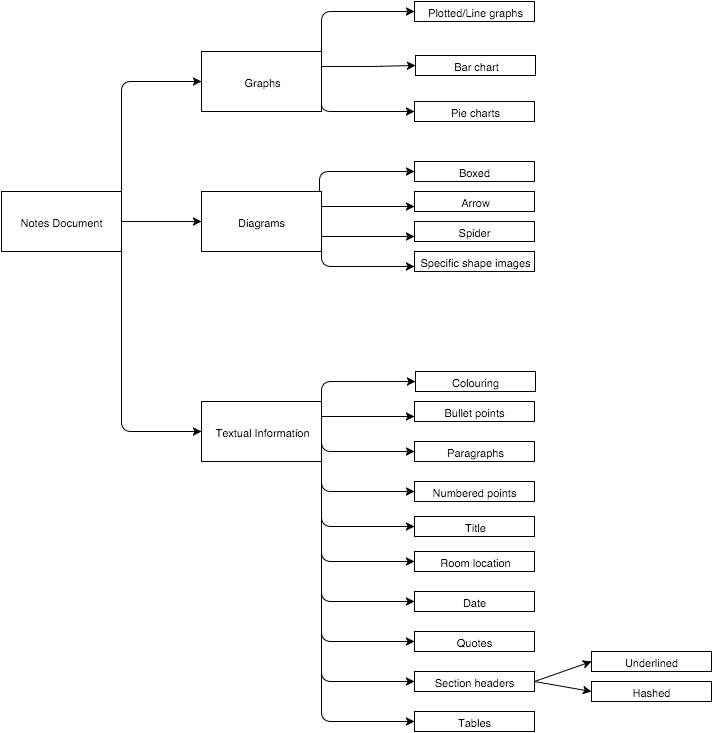
\includegraphics[scale=0.5]{images/taxonomy}
\centering
\caption{A taxonomy showing the structure and classification of different types of notes and what is contained in a note.}
 \label{fig:taxonomyofnotes}
\end{figure}

In figure \ref{fig:taxonomyofnotes}, it shows a taxonomy of the different aspects which may comprise to make a note. Textural descriptions form the core part of a note, this is essentially the important content that a note-taker is trying to remember and write down. Different note-takers form their notes in different ways, for example the headings may be underlined or hashed - if they were adopting a mark-down style approach. These sections helps to show that there's a break in the content, and should be sub-sectioned. Textural points that are short, but important, are often characterised by a colon or a bullet point; these are the most common form of concise note building, in the classisifcation. Coloured highlighting if often used for a variety of reasons: it stands out on the page and for some people colour retention is better. Finally, tables help to represent textual content in tabular form.  This is often good in notes for comparisons. 

Graphs are great visual tools for user's in helping to convery textual information in a graphical form. Naturally, they have their limitations such as they come in different shapes and sizes, such as a line-graph, pie chart or a bar chart. Coupled with graphs, notes often consist of diagram drawings.  In figure \ref{fig:taxonomyofnotes}, there are different sections and classsifications of a diagram: boxed, arrow etc. Each one has its own purpose and arrowed and box can overlap; UML diagrams are a case of this. Spider diagrams are probably the hardest to represent, due to the varying sizes and whether the user draws circles or clouds. Furthermore, specific shape diagrams are conceptutally hard to think about as it depends on the domain in which the user is drawing the note. For example, a person in biology may draw a stick person, whereas someone in Computer Science may draw a PC. 

Overall, identifying the taxonomy of notes is important as it gives context to which the application can potentially parse and identify these different classifications. Additionally, it acknowledges where there may need to be constraints due to the variations in notes and how it can deal with semi-structured documents.

% Add some more from the stuff Hannah made us write about in the first week.



\subsection{Similar Systems}
With note-taking on digital devices becoming more of the normal then software tools have been created which help users to write their notes down, edit. These are mainly WYSIWYG (What you see is what you get) editors - which a great deal of flexibility. When evaluating existing systems two were commonly used and they were: 
\begin{itemize}
  \item OneNote
  \item EverNote
  \item Google Keep
\end{itemize}

\subsubsection{OneNote}
OneNote is a note-taking and organisational application made by Microsoft  \cite{citeulike:onenote}. Commonly, this is a WYSIWG allowing you to add text, photos, drag and drop photos. This offers a wide-range of flexibility when making notes. In recent times, OneNote has developed functionality to analyse a user's handwriting, from say a stylus, and interpret the text they entered [CITE]. [CITE] In OneNote you can insert a note into document and then it would interpret the text from the note. They offer a wide range of product support from mobile based applications to web versions of their software. Office Lens [CITE] can be used in conjunction with the OneNote to help to take photos and automatically crop the image and then save them to OneNote. This feature is important and should be considered when thinking about \textit{MapMyNotes} application. The process requires you to have a microsoft account, which you sign in with. Once in they format their documents as a series of ``notebooks'' which group together similar notes. When editing notes in the input boxes then it does automatic saving behind the scenes, so you never have to click a save button. When using OneNote it feels very much like Microsoft Word - with the similar layout that gives most users a similar user experience feel.

\subsubsection{EverNote}
EverNote is a note-taking and note organisation app, it is both supported on the web and in app form. EverNote is widely used and would provide a lot of the functionality a user would need to upload their note. They have realeased development articles [CITE-2013 one] stating that they are able to do OCR recognition on images. This would allow the user to upload an image and it would give a list of words, which it thinks is the word identified. This differs from MapMyNotes where the author aims to develop an application which would give a 1-1 word comparision, rather than a list of words. Like OneNote, the notes are collated into Notebooks, offering a WYSIWG editor, giving you full control of the content that you type in. When uploading an image, to the web version, it gives you the option to edit the PDF and images, however it seems as though you have to download another application, specific to your platform,  to do this functionality. According to the website, it does to OCR recognition, however whilst using the application I could not find an easy way in the user interface to get the any text or event find out what a word was. This is something which is important and key for \textit{MapMyNotes}. Additionally, there seemed to be no way to save the note to a calendar item - only the option to send via a link. 
\subsubsection{Google Keep}
Google Keep [CITE] is a note taking application made by Google with mobile and website support. Google keep allows a user to attach an image to their note and attempt to extract the text from an image and save this in the body of the text. It allows you to tag a title, and add an associated body. This is note a WYSIWYG editor, it's a plain old text box which a user can input information into. They have the option of a remind me functionality, which will get synced to their calendar as a reminder - but there's no easy way to add it to a calendar event. Google keep seems as though it's more for TODO lists and jotting down quick notes, rather than an archiving tool suitable for note taking. Although, the tagging with labels is a nice feature  and the filter by image is a smart tool - to only show notes with images. The simplicity of the user interface and the ease in which text could be extract provides good thought going forward.

\begin{flushleft}
These three existing products are widely used by the every day note taker. They have been developed to a high quality and give the user a full control experience of what their notes can consist of. The automatically cropping of an image is an important process and should be considered when for the application going forward. \textit{MapMyNotes} aims to try and give the user full control of their lecture notes content, so that they can find their notes easily again. 
\end{flushleft}


\subsection{Personal Interest}
The author has a motivation for a project which can integrate with a calendar and automatically store notes. Notes are often written up but discarded soon after the lecture and not found until weeks before an assignment or examination is due. There is then a frenzy to try and find all the notes for a given module which are often dispersed throughout many pages in a notebook. The tool would be useful to take a photograph on a normal phone, upload it to the software service, and then attach any associated meta-data and save it to a calendar.  This would help to reduce the chance of lost notes and notes which are unreadable or split due to page breaks. Additionally, with it being in the calendar all notes will be associated to an event so quickly searching for associated notes on a calendar item would return the correct notes easily. This would reduce the time spent searching for notes and actually finding the note again and getting on with the purpose in hand.

\section{Analysis}
%Taking into account the problem and what you learned from the background work, what was your analysis of the problem? How did your analysis help to decompose the problem into the main tasks that you would undertake? Were there alternative approaches? Why did you choose one approach compared to the alternatives?

%In most cases, the agreed objectives or requirements will be the result of a compromise between what would ideally have been produced and what was felt to be possible in the time available. A discussion of the process of arriving at the final list is usually appropriate.

Due to the project originally being proposed by Dr Harry Strange, meetings were arranged before he left the department, to discuss what his initial ideas were of the application. It was here that it was confirmed with the author's personal interests, that this was a problem that needed to be solved. Looking at the existing systems it was clear what a good system would entail. The problem highlighted that there needed to be an application, which would allow you to upload a note to the application and view it and ensure that it saves it to the calendar. 

By analysing the problem a taxonomy of notes was collated. This helped to breakdown exactly what was in a set of notes. This taxonomy gave a comprehensive analysis of what information would be available to parse from the test, as well as giving the information parsed semantic meaning. It was quickly brought up that I should potentially create a specific layout for the note so that the data can be parsed sensibly, to reduce the complexity. Additionally, this highlighted all the possible things which the application could parse. Due to text being the main component of a note, it was agreed that efforts would be focused on parsing the text. Images could have been extracted from the notes but this would not form the core aspects of the notes and was placed as a task that could be implemented in the future.  This lead to the task of investigating how to extract the text from an image.  It was agreed to look into OCR tools and find a suitable tool for the application - there could have been the approach of writing my own handwriting recognition tool using Machine Learning, but that would not solve the problem it would only help to solve part of the problem as a result it was agreed the application was more importnt than this research, so an OCR tool was agreed to be used.

From the Google Keep example, it was clear that analysising the text would be an imperitive part of the application, this lead to the task of having to work out of a way to analyse characters on the image. Initially, the idea was to analyse all the characters on the page and parse them, like Google Keep, however this would be far too complex. Due to the complexity this had to be scaled back and we would have to analyse the meta-data from the note, i.e: Title, lecturer, date etc, this became the primary aim of the tool. Additionally, due to analysing handwriting being a complicated process to begin with then it was agreed that it would only be trained on the author's handwriting,  with the possibility of extending it in the future - this was chosen due to help reduce the complexity of the application and simplify the process within the timeframe.

In addition to this, it was clear that when trying to analyse the image a certain structure would have to be applied to the notes to help to aid suggestions. As a result a set of rules would have to be collated to ensure all notes were structured in this way when using the application. As already mentioned, this would help to ease the complexity of parsing the notes and reduce the need for Natural Language processing, which would increase the complexity of the application again beyond the ability to complete it in the timeframe. 

During the meeting with Dr Harry Strange, it was clear that the tool would need to be used on the go, potentially where a laptop access was reduced. Trying to make the application available to everyone a web application as a software as a service, would be created. This was chosen instead of a mobile application due to the accessibility which a web application can give you - especially if it's responsive. Additionally, from the background research conducted all three of the afformentioned products have accompanying web applications.

Next it was discussed what the web application should actually do. From looking at the applications, it was clear that a view all notes, search and add-edit , delete (the usual CRUD application) would be needed to help to make a full system; all the examples looked at contained this functionality so it was important that I acknowledged that this was an important thing. Reflecting on the premise of the application it was analysed that the best way to search for notes would be by module code, as most University students would want to find specific module notes. This created the tasks of being able to search for the module code and show all codes for that user. 

One thing that was noticed very quickly, from the research, was a lack of calendar integration. Reflecting on the conversations with Dr Harry Strange, this was an important feature for him. The challenge of deciding which calendar to integrate with was an important decision. From a survey [CITE SURVEY] Google calendar is considered to the most popular app - so it was decided that Google calendar integration was needed. Other calendars such as Microsoft's calendar was considered but realistically there was only time to implement one calendar integration. Therefore, the application had to save a url of the saved note to the calendar event for the given day the user enters.

%There should be a clear statement of the objectives of the work, which you will evaluate at the end of the work.
\subsection{Objectives}
As a result of the analysis of the problem, the following high-level requirements were formulated:
\begin{enumerate}
	\item Investigate how to extract handwriting text from an image - this will involve looking into ways OCR tools can interpret handwriting. 
	\item Train the OCR to recognise text of the author's handwriting.
	\item Produce a set of a rules which a note must comply to.
	\item Produce a web application to form the core part of the product. This includes allowing a user to upload an image, display the image. Add appropriate tagging to a note such as module code. 
	\item The user must be able to search for a given module code, shwoing the fill list of notes based on the module code entered.
	\item The backend of the application must conduct basic OCR recognition, analysing the first 3 lines of the notes. 
	\item The backend must integrate with a calendar to archive the notes away later to be found again.
\end{enumerate}

Ideally, having image extraction and making it into a WSIWYG editor, like OneNote, would have been the desired outcome from the application. This would incorporate the analysis of the text from the image as a whole and display coloured text. After discussions with my supervisor, Dr Hannah Dee, it was clearly stated that this was far too complex for the timeframe so a re-think had to be conducted. Initially, my supervisor thought that the web application , excluding any OCR recognition, would be suitable for a minimal product and a dissertation. Although this was sensible, 

During the first few meetings my supervisor, Dr Hannah Dee, it was discussed what was actually plausable in the time frame. Acknowledging that the project was large and could be expanded we opted to rein in the features and get a minimal project. Dr Hannah Dee suggested that the just the application without the Tesseract parsing would be enough for a minimal product, however I wanted the ability to try and recognise handwriting recognition. So we comprised but mentioned that the handwriting recognition would be a background process, and not the main aim.

\section{Process}
%You need to describe briefly the life cycle model or research method that you used. You do not need to write about all of the different process models that you are aware of. Focus on the process model that you have used. It is possible that you needed to adapt an existing process model to suit your project; clearly identify what you used and how you adapted it for your needs.
Software projects tends to have a degree of uncertainty regarding their full end outcome regarding requirements. \textit{MapMyNotes} has a great deal of uncertainty regarding how long certain tasks would take, as well as thinking of new functionality from customer meetings and user testing feedback.  Tasks such as training the author's handwriting could not be truely estimated due on a Gantt chart due to a degree of uncertainty regarding how long it would take. As a result, a plan-driven approach, such as the Waterfall model, would not be suitable for this project where the requirements may change from week to week. Instead, an Agile approach was followed throughout the process. 

Scrum[CITE] is normally a methodology for teams to help to guide a team to be the most productive as possible. Due to this being a single person project the Scrum approach has to be modified to work in this scenario. Work to be completed is separated into sprints, which shows what work needs to be completed in the sprint. Sprints can vary from 1 - 4 weeks in length but a shorter sprint allows feedback to be gotten back to a team quicker, allowing more change to occur.  Scrum uses user stories to help to make sure the team is always doing client-valued work - these stories are collated and put into a backlog, which forms a list of all the user stories for the project. At the start of each sprint user-stories are pulled from the backlog and placed into the sprint, each one estimated. At the end of the sprint a review and retrospective is conducted to analyse the sprint, identify what was good and what was not so good so the next sprint can be improved.

For the single person project, this methology was used and adapted. Sprints in the project were a week long, which coincided with the weekly supervisor meeting on a Thursday.  A backlog was collated at the start of the project to reflect the initial stories. These were summarised as epics (a high level interpretation of a story). Each story was estimated accordingly not on time, but on the level of complexity it would take to complete the task. The tasks were estimated against a ``goldilock'' task, which is a base task which all other tasks are estimated around. I.e, if you estimate that the complexity of the research Flask's routing system is a 5, all other tasks will be compared against this for complexity. During the planning stages I adopted the planning poker [CITE] technique; user-stories are estimated on a scale of 1, 2, 3, 5, 8 and so on. If a task was usually 15 or above then it would be reflected upon to ensure that I fully understood the scope of the task and where it needs to be broken down into smaller tasks which would reduce the complexity of the overall task.  At the end of the sprint a review and retrospective was conducted, instead of face to face with a team it was a reflection in the form of a blog post [CITE WEBSITE]. These were used to reflect on what has been achieved in the sprint, what went well and should be continues and what could be improved upon in the next sprint.  Furthermore, I used this reflection to do some pre-planning, after my meeting with my supervisor, to decide what would be brought into the sprint currently. At the end of every sprint, a conversation between myself and my supervisor was utilised to determine what needed to be completed in the next sprint. Once we had decided the user stories which matched, at maximum, the last sprints story points were brought forward to the sprint. For example, if 20 story points were completed in sprint 3, then 20 story points would be allocated for sprint 4 and the user stories brought in would have to add up to 20 points. The project was managed on the open source management tool Taiga.io [CITE] which was invaluable, and provided built in functionality such as burndown charts per sprint, which show how well you're completing story points and tasks. These were used in the sprint to analyse how well work was being completed.

Coupled with Scrum, there was a modification to the development process to incorporate Extreme Programming principles[CITE EXTREME PROGRAMMING]. Principles such as: merciless refactoring, continuous integration and test-driven development were used.  Test-driven development (TDD) is the art of writing the tests prior to writing the code. Using this principles ensures that tests were written for functions and methods, as well as helping to think about the design prior to the implementation. [CITE] agrees that tests an additional form of documentation. With TDD it follows three cycles: Red, a failing test, green, a passing task, refactor, refactoring the design. The aim is to do the minimal design needed to pass the test; this approach was adopted throughout the project. 

Continous Integration tools were a core part of the process and life cycle on this project. When the code was pushed to the repository a build script was triggered in the continous integration software to build and test all the system to ensure they worked in an isolated environment. Finally, CRC cards [CITE] were used during the design section to consider how implementation between systems would interact and how different classes would look and feel. This principle from Extreme Programming helped to keep the design simple and not convoluted for the task, focussing on the current task.